\documentclass{standalone}
\usepackage{tikz}
\usetikzlibrary{patterns, positioning}

\begin{document}
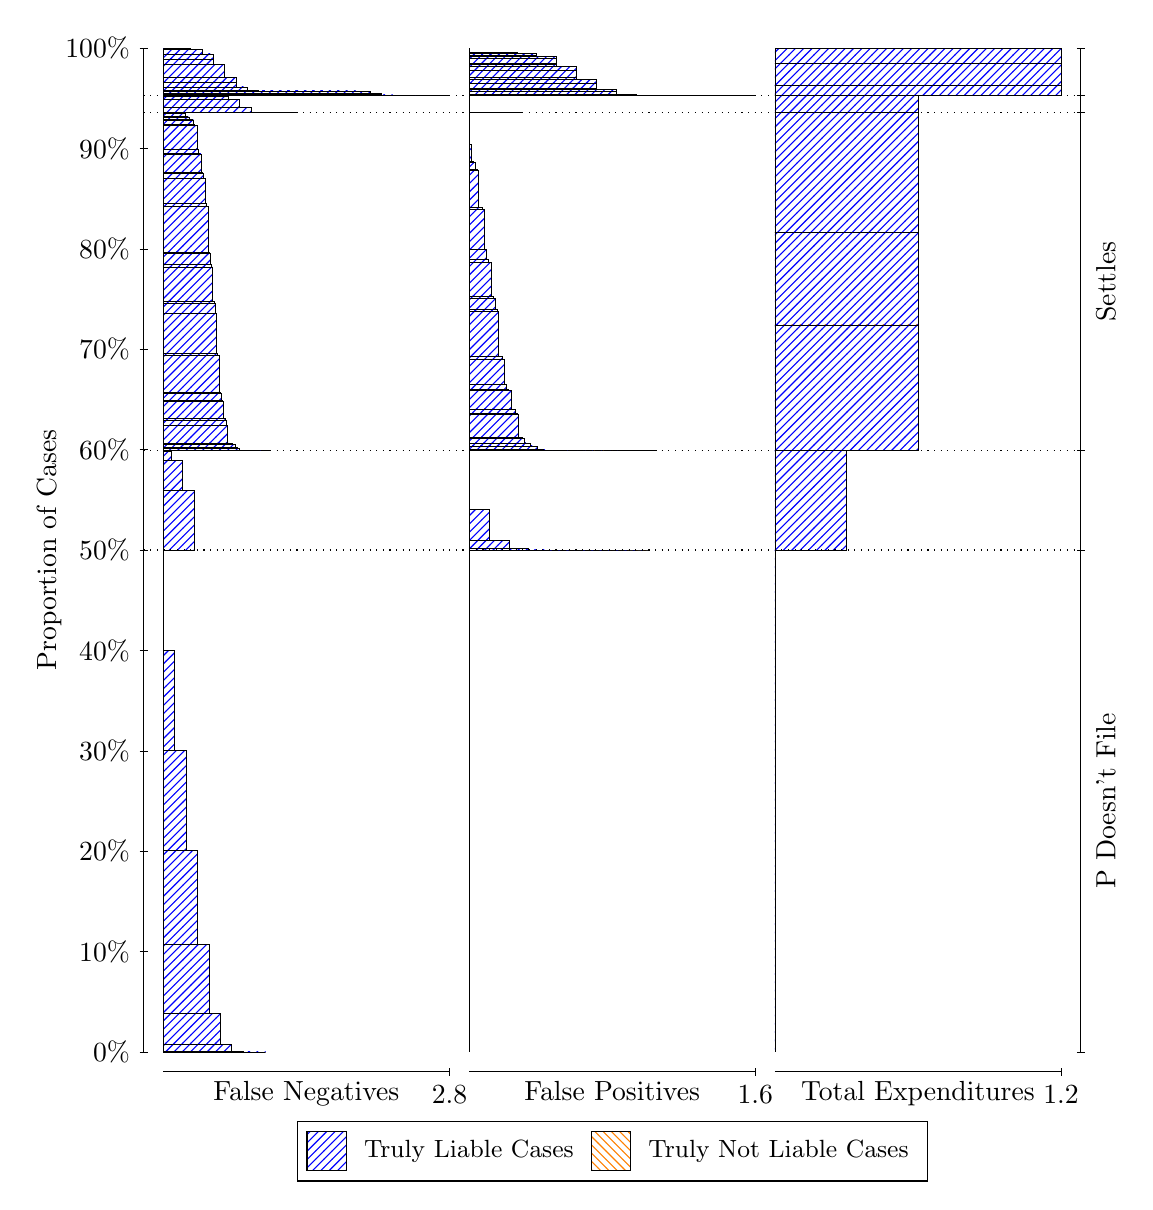
\begin{tikzpicture}
\draw[black, very thin] (1.5,1.75) -- (1.5,14.5);
\node[rotate=90, anchor=center] at (0.3, 8.125) {Proportion of Cases};
\draw[black, very thin] (1.45,1.75) -- (1.55,1.75);
\node[anchor=east] at (1.45, 1.75) {0\%};
\draw[black, very thin] (1.45,3.025) -- (1.55,3.025);
\node[anchor=east] at (1.45, 3.025) {10\%};
\draw[black, very thin] (1.45,4.3) -- (1.55,4.3);
\node[anchor=east] at (1.45, 4.3) {20\%};
\draw[black, very thin] (1.45,5.575) -- (1.55,5.575);
\node[anchor=east] at (1.45, 5.575) {30\%};
\draw[black, very thin] (1.45,6.85) -- (1.55,6.85);
\node[anchor=east] at (1.45, 6.85) {40\%};
\draw[black, very thin] (1.45,8.125) -- (1.55,8.125);
\node[anchor=east] at (1.45, 8.125) {50\%};
\draw[black, very thin] (1.45,9.4) -- (1.55,9.4);
\node[anchor=east] at (1.45, 9.4) {60\%};
\draw[black, very thin] (1.45,10.675) -- (1.55,10.675);
\node[anchor=east] at (1.45, 10.675) {70\%};
\draw[black, very thin] (1.45,11.95) -- (1.55,11.95);
\node[anchor=east] at (1.45, 11.95) {80\%};
\draw[black, very thin] (1.45,13.225) -- (1.55,13.225);
\node[anchor=east] at (1.45, 13.225) {90\%};
\draw[black, very thin] (1.45,14.5) -- (1.55,14.5);
\node[anchor=east] at (1.45, 14.5) {100\%};

\draw[black, very thin] (13.4,1.75) -- (13.4,14.5);
\draw[black, very thin] (13.35,1.75) -- (13.45,1.75);
\node[anchor=west] at (13.35, 1.75) {};
\draw[black, very thin] (13.35,8.125) -- (13.45,8.125);
\node[anchor=west] at (13.35, 8.125) {};
\draw[black, very thin] (13.35,9.3926) -- (13.45,9.3926);
\node[anchor=west] at (13.35, 9.3926) {};
\draw[black, very thin] (13.35,13.68) -- (13.45,13.68);
\node[anchor=west] at (13.35, 13.68) {};
\draw[black, very thin] (13.35,13.898) -- (13.45,13.898);
\node[anchor=west] at (13.35, 13.898) {};
\draw[black, very thin] (13.35,14.5) -- (13.45,14.5);
\node[anchor=west] at (13.35, 14.5) {};

\draw[black, very thin, pattern color=blue, pattern=north east lines] (1.75,1.75) rectangle (3.0476,1.75);
\draw[black, very thin, pattern color=blue, pattern=north east lines] (1.75,1.75) rectangle (2.9034,1.7503);
\draw[black, very thin, pattern color=blue, pattern=north east lines] (1.75,1.7503) rectangle (2.7593,1.7583);
\draw[black, very thin, pattern color=blue, pattern=north east lines] (1.75,1.7583) rectangle (2.6151,1.8435);
\draw[black, very thin, pattern color=blue, pattern=north east lines] (1.75,1.8435) rectangle (2.4709,2.2369);
\draw[black, very thin, pattern color=blue, pattern=north east lines] (1.75,2.2369) rectangle (2.3267,3.1185);
\draw[black, very thin, pattern color=blue, pattern=north east lines] (1.75,3.1185) rectangle (2.1825,4.3083);
\draw[black, very thin, pattern color=blue, pattern=north east lines] (1.75,4.3083) rectangle (2.0384,5.5753);
\draw[black, very thin, pattern color=blue, pattern=north east lines] (1.75,5.5753) rectangle (1.8942,6.85);
\draw[black, very thin, pattern color=orange, pattern=north west lines] (1.75,6.85) rectangle (1.75,6.85);
\draw[black, very thin, pattern color=blue, pattern=north east lines] (1.75,6.85) rectangle (1.75,8.125);
\draw[black, very thin, pattern color=blue, pattern=north east lines] (1.75,8.125) rectangle (2.1393,8.8794);
\draw[black, very thin, pattern color=blue, pattern=north east lines] (1.75,8.8794) rectangle (1.9951,9.2662);
\draw[black, very thin, pattern color=blue, pattern=north east lines] (1.75,9.2662) rectangle (1.8509,9.3769);
\draw[black, very thin, pattern color=orange, pattern=north west lines] (1.75,9.3769) rectangle (1.75,9.3769);
\draw[black, very thin, pattern color=blue, pattern=north east lines] (1.75,9.3769) rectangle (1.75,9.3926);
\draw[black, very thin, pattern color=blue, pattern=north east lines] (1.75,9.3926) rectangle (3.1125,9.3926);
\draw[black, very thin, pattern color=blue, pattern=north east lines] (1.75,9.3926) rectangle (3.0476,9.3926);
\draw[black, very thin, pattern color=blue, pattern=north east lines] (1.75,9.3926) rectangle (2.9827,9.3926);
\draw[black, very thin, pattern color=blue, pattern=north east lines] (1.75,9.3926) rectangle (2.9683,9.3926);
\draw[black, very thin, pattern color=blue, pattern=north east lines] (1.75,9.3926) rectangle (2.9179,9.3926);
\draw[black, very thin, pattern color=blue, pattern=north east lines] (1.75,9.3926) rectangle (2.9034,9.3926);
\draw[black, very thin, pattern color=blue, pattern=north east lines] (1.75,9.3926) rectangle (2.853,9.3935);
\draw[black, very thin, pattern color=blue, pattern=north east lines] (1.75,9.3935) rectangle (2.8386,9.3937);
\draw[black, very thin, pattern color=blue, pattern=north east lines] (1.75,9.3937) rectangle (2.8241,9.3937);
\draw[black, very thin, pattern color=blue, pattern=north east lines] (1.75,9.3937) rectangle (2.7881,9.3938);
\draw[black, very thin, pattern color=blue, pattern=north east lines] (1.75,9.3938) rectangle (2.7737,9.394);
\draw[black, very thin, pattern color=blue, pattern=north east lines] (1.75,9.394) rectangle (2.7593,9.3941);
\draw[black, very thin, pattern color=blue, pattern=north east lines] (1.75,9.3941) rectangle (2.7232,9.3942);
\draw[black, very thin, pattern color=blue, pattern=north east lines] (1.75,9.3942) rectangle (2.7088,9.4188);
\draw[black, very thin, pattern color=blue, pattern=north east lines] (1.75,9.4188) rectangle (2.6944,9.4268);
\draw[black, very thin, pattern color=blue, pattern=north east lines] (1.75,9.4268) rectangle (2.68,9.4295);
\draw[black, very thin, pattern color=blue, pattern=north east lines] (1.75,9.4295) rectangle (2.6583,9.4691);
\draw[black, very thin, pattern color=blue, pattern=north east lines] (1.75,9.4691) rectangle (2.6439,9.4708);
\draw[black, very thin, pattern color=blue, pattern=north east lines] (1.75,9.4708) rectangle (2.6295,9.4812);
\draw[black, very thin, pattern color=blue, pattern=north east lines] (1.75,9.4812) rectangle (2.6151,9.4839);
\draw[black, very thin, pattern color=blue, pattern=north east lines] (1.75,9.4839) rectangle (2.579,9.4861);
\draw[black, very thin, pattern color=blue, pattern=north east lines] (1.75,9.4861) rectangle (2.5646,9.7044);
\draw[black, very thin, pattern color=blue, pattern=north east lines] (1.75,9.7044) rectangle (2.5502,9.7732);
\draw[black, very thin, pattern color=blue, pattern=north east lines] (1.75,9.7732) rectangle (2.5358,9.7945);
\draw[black, very thin, pattern color=blue, pattern=north east lines] (1.75,9.7945) rectangle (2.5142,10.01);
\draw[black, very thin, pattern color=blue, pattern=north east lines] (1.75,10.01) rectangle (2.4997,10.026);
\draw[black, very thin, pattern color=blue, pattern=north east lines] (1.75,10.026) rectangle (2.4853,10.111);
\draw[black, very thin, pattern color=blue, pattern=north east lines] (1.75,10.111) rectangle (2.4709,10.128);
\draw[black, very thin, pattern color=blue, pattern=north east lines] (1.75,10.128) rectangle (2.4637,10.598);
\draw[black, very thin, pattern color=blue, pattern=north east lines] (1.75,10.598) rectangle (2.4349,10.618);
\draw[black, very thin, pattern color=blue, pattern=north east lines] (1.75,10.618) rectangle (2.4204,11.128);
\draw[black, very thin, pattern color=blue, pattern=north east lines] (1.75,11.128) rectangle (2.406,11.259);
\draw[black, very thin, pattern color=blue, pattern=north east lines] (1.75,11.259) rectangle (2.3916,11.29);
\draw[black, very thin, pattern color=blue, pattern=north east lines] (1.75,11.29) rectangle (2.37,11.721);
\draw[black, very thin, pattern color=blue, pattern=north east lines] (1.75,11.721) rectangle (2.3556,11.751);
\draw[black, very thin, pattern color=blue, pattern=north east lines] (1.75,11.751) rectangle (2.3411,11.893);
\draw[black, very thin, pattern color=blue, pattern=north east lines] (1.75,11.893) rectangle (2.3267,11.91);
\draw[black, very thin, pattern color=blue, pattern=north east lines] (1.75,11.91) rectangle (2.3195,12.487);
\draw[black, very thin, pattern color=blue, pattern=north east lines] (1.75,12.487) rectangle (2.2907,12.527);
\draw[black, very thin, pattern color=blue, pattern=north east lines] (1.75,12.527) rectangle (2.2763,12.849);
\draw[black, very thin, pattern color=blue, pattern=north east lines] (1.75,12.849) rectangle (2.2618,12.909);
\draw[black, very thin, pattern color=blue, pattern=north east lines] (1.75,12.909) rectangle (2.2474,12.918);
\draw[black, very thin, pattern color=blue, pattern=north east lines] (1.75,12.918) rectangle (2.2258,13.155);
\draw[black, very thin, pattern color=blue, pattern=north east lines] (1.75,13.155) rectangle (2.2114,13.166);
\draw[black, very thin, pattern color=blue, pattern=north east lines] (1.75,13.166) rectangle (2.197,13.215);
\draw[black, very thin, pattern color=blue, pattern=north east lines] (1.75,13.215) rectangle (2.1825,13.218);
\draw[black, very thin, pattern color=blue, pattern=north east lines] (1.75,13.218) rectangle (2.1753,13.515);
\draw[black, very thin, pattern color=blue, pattern=north east lines] (1.75,13.515) rectangle (2.1465,13.529);
\draw[black, very thin, pattern color=blue, pattern=north east lines] (1.75,13.529) rectangle (2.1321,13.586);
\draw[black, very thin, pattern color=blue, pattern=north east lines] (1.75,13.586) rectangle (2.1177,13.592);
\draw[black, very thin, pattern color=blue, pattern=north east lines] (1.75,13.592) rectangle (2.1032,13.593);
\draw[black, very thin, pattern color=blue, pattern=north east lines] (1.75,13.593) rectangle (2.0816,13.624);
\draw[black, very thin, pattern color=blue, pattern=north east lines] (1.75,13.624) rectangle (2.0672,13.625);
\draw[black, very thin, pattern color=blue, pattern=north east lines] (1.75,13.625) rectangle (2.0528,13.629);
\draw[black, very thin, pattern color=blue, pattern=north east lines] (1.75,13.629) rectangle (2.0384,13.629);
\draw[black, very thin, pattern color=blue, pattern=north east lines] (1.75,13.629) rectangle (2.0312,13.673);
\draw[black, very thin, pattern color=blue, pattern=north east lines] (1.75,13.673) rectangle (2.0023,13.674);
\draw[black, very thin, pattern color=blue, pattern=north east lines] (1.75,13.674) rectangle (1.9879,13.677);
\draw[black, very thin, pattern color=blue, pattern=north east lines] (1.75,13.677) rectangle (1.9735,13.677);
\draw[black, very thin, pattern color=blue, pattern=north east lines] (1.75,13.677) rectangle (1.9591,13.677);
\draw[black, very thin, pattern color=blue, pattern=north east lines] (1.75,13.677) rectangle (1.9374,13.678);
\draw[black, very thin, pattern color=blue, pattern=north east lines] (1.75,13.678) rectangle (1.923,13.678);
\draw[black, very thin, pattern color=blue, pattern=north east lines] (1.75,13.678) rectangle (1.9086,13.678);
\draw[black, very thin, pattern color=blue, pattern=north east lines] (1.75,13.678) rectangle (1.8942,13.678);
\draw[black, very thin, pattern color=blue, pattern=north east lines] (1.75,13.678) rectangle (1.887,13.68);
\draw[black, very thin, pattern color=blue, pattern=north east lines] (1.75,13.68) rectangle (1.8581,13.68);
\draw[black, very thin, pattern color=blue, pattern=north east lines] (1.75,13.68) rectangle (1.8437,13.68);
\draw[black, very thin, pattern color=blue, pattern=north east lines] (1.75,13.68) rectangle (1.8293,13.68);
\draw[black, very thin, pattern color=blue, pattern=north east lines] (1.75,13.68) rectangle (1.8149,13.68);
\draw[black, very thin, pattern color=blue, pattern=north east lines] (1.75,13.68) rectangle (1.7933,13.68);
\draw[black, very thin, pattern color=blue, pattern=north east lines] (1.75,13.68) rectangle (1.7788,13.68);
\draw[black, very thin, pattern color=blue, pattern=north east lines] (1.75,13.68) rectangle (1.7644,13.68);
\draw[black, very thin, pattern color=orange, pattern=north west lines] (1.75,13.68) rectangle (1.75,13.68);
\draw[black, very thin, pattern color=blue, pattern=north east lines] (1.75,13.68) rectangle (1.75,13.68);
\draw[black, very thin, pattern color=blue, pattern=north east lines] (1.75,13.68) rectangle (3.4369,13.68);
\draw[black, very thin, pattern color=blue, pattern=north east lines] (1.75,13.68) rectangle (3.2927,13.68);
\draw[black, very thin, pattern color=blue, pattern=north east lines] (1.75,13.68) rectangle (3.1485,13.68);
\draw[black, very thin, pattern color=blue, pattern=north east lines] (1.75,13.68) rectangle (3.0044,13.687);
\draw[black, very thin, pattern color=blue, pattern=north east lines] (1.75,13.687) rectangle (2.8602,13.746);
\draw[black, very thin, pattern color=blue, pattern=north east lines] (1.75,13.746) rectangle (2.716,13.848);
\draw[black, very thin, pattern color=blue, pattern=north east lines] (1.75,13.848) rectangle (2.5718,13.892);
\draw[black, very thin, pattern color=blue, pattern=north east lines] (1.75,13.892) rectangle (2.4276,13.898);
\draw[black, very thin, pattern color=blue, pattern=north east lines] (1.75,13.898) rectangle (2.2835,13.898);
\draw[black, very thin, pattern color=blue, pattern=north east lines] (1.75,13.898) rectangle (2.1393,13.898);
\draw[black, very thin, pattern color=orange, pattern=north west lines] (1.75,13.898) rectangle (1.75,13.898);
\draw[black, very thin, pattern color=blue, pattern=north east lines] (1.75,13.898) rectangle (5.3833,13.898);
\draw[black, very thin, pattern color=blue, pattern=north east lines] (1.75,13.898) rectangle (5.2392,13.898);
\draw[black, very thin, pattern color=blue, pattern=north east lines] (1.75,13.898) rectangle (5.095,13.898);
\draw[black, very thin, pattern color=blue, pattern=north east lines] (1.75,13.898) rectangle (4.9508,13.898);
\draw[black, very thin, pattern color=blue, pattern=north east lines] (1.75,13.898) rectangle (4.9508,13.898);
\draw[black, very thin, pattern color=blue, pattern=north east lines] (1.75,13.898) rectangle (4.8066,13.899);
\draw[black, very thin, pattern color=blue, pattern=north east lines] (1.75,13.899) rectangle (4.6624,13.903);
\draw[black, very thin, pattern color=blue, pattern=north east lines] (1.75,13.903) rectangle (4.6624,13.904);
\draw[black, very thin, pattern color=blue, pattern=north east lines] (1.75,13.904) rectangle (4.5183,13.915);
\draw[black, very thin, pattern color=blue, pattern=north east lines] (1.75,13.915) rectangle (4.5183,13.922);
\draw[black, very thin, pattern color=blue, pattern=north east lines] (1.75,13.922) rectangle (4.3741,13.947);
\draw[black, very thin, pattern color=blue, pattern=north east lines] (1.75,13.947) rectangle (4.2299,13.954);
\draw[black, very thin, pattern color=blue, pattern=north east lines] (1.75,13.954) rectangle (4.2299,13.956);
\draw[black, very thin, pattern color=blue, pattern=north east lines] (1.75,13.956) rectangle (4.0857,13.956);
\draw[black, very thin, pattern color=blue, pattern=north east lines] (1.75,13.956) rectangle (3.9415,13.956);
\draw[black, very thin, pattern color=blue, pattern=north east lines] (1.75,13.956) rectangle (3.7974,13.956);
\draw[black, very thin, pattern color=blue, pattern=north east lines] (1.75,13.956) rectangle (3.7974,13.956);
\draw[black, very thin, pattern color=blue, pattern=north east lines] (1.75,13.956) rectangle (3.6532,13.956);
\draw[black, very thin, pattern color=blue, pattern=north east lines] (1.75,13.956) rectangle (3.5378,13.956);
\draw[black, very thin, pattern color=blue, pattern=north east lines] (1.75,13.956) rectangle (3.509,13.956);
\draw[black, very thin, pattern color=blue, pattern=north east lines] (1.75,13.956) rectangle (3.3937,13.956);
\draw[black, very thin, pattern color=blue, pattern=north east lines] (1.75,13.956) rectangle (3.2495,13.956);
\draw[black, very thin, pattern color=blue, pattern=north east lines] (1.75,13.956) rectangle (3.1053,13.956);
\draw[black, very thin, pattern color=blue, pattern=north east lines] (1.75,13.956) rectangle (3.1053,13.956);
\draw[black, very thin, pattern color=blue, pattern=north east lines] (1.75,13.956) rectangle (2.9611,13.959);
\draw[black, very thin, pattern color=blue, pattern=north east lines] (1.75,13.959) rectangle (2.9611,13.962);
\draw[black, very thin, pattern color=blue, pattern=north east lines] (1.75,13.962) rectangle (2.8169,14.007);
\draw[black, very thin, pattern color=blue, pattern=north east lines] (1.75,14.007) rectangle (2.6728,14.069);
\draw[black, very thin, pattern color=blue, pattern=north east lines] (1.75,14.069) rectangle (2.6728,14.131);
\draw[black, very thin, pattern color=blue, pattern=north east lines] (1.75,14.131) rectangle (2.5286,14.295);
\draw[black, very thin, pattern color=blue, pattern=north east lines] (1.75,14.295) rectangle (2.3844,14.358);
\draw[black, very thin, pattern color=blue, pattern=north east lines] (1.75,14.358) rectangle (2.3844,14.361);
\draw[black, very thin, pattern color=blue, pattern=north east lines] (1.75,14.361) rectangle (2.3844,14.425);
\draw[black, very thin, pattern color=blue, pattern=north east lines] (1.75,14.425) rectangle (2.2402,14.482);
\draw[black, very thin, pattern color=blue, pattern=north east lines] (1.75,14.482) rectangle (2.2402,14.484);
\draw[black, very thin, pattern color=blue, pattern=north east lines] (1.75,14.484) rectangle (2.096,14.489);
\draw[black, very thin, pattern color=blue, pattern=north east lines] (1.75,14.489) rectangle (2.096,14.49);
\draw[black, very thin, pattern color=blue, pattern=north east lines] (1.75,14.49) rectangle (2.096,14.498);
\draw[black, very thin, pattern color=blue, pattern=north east lines] (1.75,14.498) rectangle (1.9519,14.5);
\draw[black, very thin, pattern color=blue, pattern=north east lines] (1.75,14.5) rectangle (1.9519,14.5);
\draw[black, very thin, pattern color=blue, pattern=north east lines] (1.75,14.5) rectangle (1.8077,14.5);
\draw[black, very thin, pattern color=blue, pattern=north east lines] (1.75,14.5) rectangle (1.8077,14.5);
\draw[black, very thin, pattern color=orange, pattern=north west lines] (1.75,14.5) rectangle (1.75,14.5);
\draw[black, very thin, pattern color=blue, pattern=north east lines] (1.75,14.5) rectangle (1.75,14.5);
\draw[black, very thin, pattern color=orange, pattern=north west lines] (5.6333,1.75) rectangle (5.6333,1.75);
\draw[black, very thin, pattern color=blue, pattern=north east lines] (5.6333,1.75) rectangle (5.6333,8.125);
\draw[black, very thin, pattern color=orange, pattern=north west lines] (5.6333,8.125) rectangle (7.9042,8.125);
\draw[black, very thin, pattern color=blue, pattern=north east lines] (5.6333,8.125) rectangle (7.9042,8.125);
\draw[black, very thin, pattern color=blue, pattern=north east lines] (5.6333,8.125) rectangle (7.6519,8.125);
\draw[black, very thin, pattern color=blue, pattern=north east lines] (5.6333,8.125) rectangle (7.3995,8.125);
\draw[black, very thin, pattern color=blue, pattern=north east lines] (5.6333,8.125) rectangle (7.1472,8.125);
\draw[black, very thin, pattern color=blue, pattern=north east lines] (5.6333,8.125) rectangle (6.8949,8.125);
\draw[black, very thin, pattern color=blue, pattern=north east lines] (5.6333,8.125) rectangle (6.6426,8.1258);
\draw[black, very thin, pattern color=blue, pattern=north east lines] (5.6333,8.1258) rectangle (6.3903,8.1407);
\draw[black, very thin, pattern color=blue, pattern=north east lines] (5.6333,8.1407) rectangle (6.138,8.2513);
\draw[black, very thin, pattern color=blue, pattern=north east lines] (5.6333,8.2513) rectangle (5.8856,8.6382);
\draw[black, very thin, pattern color=blue, pattern=north east lines] (5.6333,8.6382) rectangle (5.6333,9.3926);
\draw[black, very thin, pattern color=orange, pattern=north west lines] (5.6333,9.3926) rectangle (8.0177,9.3926);
\draw[black, very thin, pattern color=blue, pattern=north east lines] (5.6333,9.3926) rectangle (8.0177,9.3926);
\draw[black, very thin, pattern color=blue, pattern=north east lines] (5.6333,9.3926) rectangle (7.7654,9.3926);
\draw[black, very thin, pattern color=orange, pattern=north west lines] (5.6333,9.3926) rectangle (7.6771,9.3926);
\draw[black, very thin, pattern color=blue, pattern=north east lines] (5.6333,9.3926) rectangle (7.6771,9.3926);
\draw[black, very thin, pattern color=orange, pattern=north west lines] (5.6333,9.3926) rectangle (7.5635,9.3926);
\draw[black, very thin, pattern color=blue, pattern=north east lines] (5.6333,9.3926) rectangle (7.5635,9.3926);
\draw[black, very thin, pattern color=blue, pattern=north east lines] (5.6333,9.3926) rectangle (7.5131,9.3926);
\draw[black, very thin, pattern color=orange, pattern=north west lines] (5.6333,9.3926) rectangle (7.45,9.3926);
\draw[black, very thin, pattern color=blue, pattern=north east lines] (5.6333,9.3926) rectangle (7.45,9.3926);
\draw[black, very thin, pattern color=blue, pattern=north east lines] (5.6333,9.3926) rectangle (7.4248,9.3926);
\draw[black, very thin, pattern color=orange, pattern=north west lines] (5.6333,9.3926) rectangle (7.3365,9.3926);
\draw[black, very thin, pattern color=blue, pattern=north east lines] (5.6333,9.3926) rectangle (7.3365,9.3926);
\draw[black, very thin, pattern color=blue, pattern=north east lines] (5.6333,9.3926) rectangle (7.3112,9.3926);
\draw[black, very thin, pattern color=blue, pattern=north east lines] (5.6333,9.3926) rectangle (7.2608,9.3926);
\draw[black, very thin, pattern color=orange, pattern=north west lines] (5.6333,9.3926) rectangle (7.2229,9.3926);
\draw[black, very thin, pattern color=blue, pattern=north east lines] (5.6333,9.3926) rectangle (7.2229,9.3926);
\draw[black, very thin, pattern color=blue, pattern=north east lines] (5.6333,9.3926) rectangle (7.1977,9.3926);
\draw[black, very thin, pattern color=blue, pattern=north east lines] (5.6333,9.3926) rectangle (7.1725,9.3926);
\draw[black, very thin, pattern color=orange, pattern=north west lines] (5.6333,9.3926) rectangle (7.1094,9.3926);
\draw[black, very thin, pattern color=blue, pattern=north east lines] (5.6333,9.3926) rectangle (7.1094,9.3926);
\draw[black, very thin, pattern color=blue, pattern=north east lines] (5.6333,9.3926) rectangle (7.0841,9.3926);
\draw[black, very thin, pattern color=blue, pattern=north east lines] (5.6333,9.3926) rectangle (7.0589,9.3926);
\draw[black, very thin, pattern color=blue, pattern=north east lines] (5.6333,9.3926) rectangle (7.0084,9.3926);
\draw[black, very thin, pattern color=orange, pattern=north west lines] (5.6333,9.3926) rectangle (6.9958,9.3926);
\draw[black, very thin, pattern color=blue, pattern=north east lines] (5.6333,9.3926) rectangle (6.9958,9.3926);
\draw[black, very thin, pattern color=blue, pattern=north east lines] (5.6333,9.3926) rectangle (6.9706,9.3926);
\draw[black, very thin, pattern color=blue, pattern=north east lines] (5.6333,9.3926) rectangle (6.9454,9.3926);
\draw[black, very thin, pattern color=blue, pattern=north east lines] (5.6333,9.3926) rectangle (6.9201,9.3926);
\draw[black, very thin, pattern color=orange, pattern=north west lines] (5.6333,9.3926) rectangle (6.8823,9.3926);
\draw[black, very thin, pattern color=blue, pattern=north east lines] (5.6333,9.3926) rectangle (6.8823,9.3926);
\draw[black, very thin, pattern color=blue, pattern=north east lines] (5.6333,9.3926) rectangle (6.8571,9.3926);
\draw[black, very thin, pattern color=blue, pattern=north east lines] (5.6333,9.3926) rectangle (6.8318,9.3926);
\draw[black, very thin, pattern color=blue, pattern=north east lines] (5.6333,9.3926) rectangle (6.8066,9.3926);
\draw[black, very thin, pattern color=blue, pattern=north east lines] (5.6333,9.3926) rectangle (6.7561,9.3942);
\draw[black, very thin, pattern color=blue, pattern=north east lines] (5.6333,9.3942) rectangle (6.7435,9.3942);
\draw[black, very thin, pattern color=blue, pattern=north east lines] (5.6333,9.3942) rectangle (6.7183,9.3943);
\draw[black, very thin, pattern color=blue, pattern=north east lines] (5.6333,9.3943) rectangle (6.6931,9.3943);
\draw[black, very thin, pattern color=blue, pattern=north east lines] (5.6333,9.3943) rectangle (6.6678,9.3953);
\draw[black, very thin, pattern color=blue, pattern=north east lines] (5.6333,9.3953) rectangle (6.63,9.3953);
\draw[black, very thin, pattern color=blue, pattern=north east lines] (5.6333,9.3953) rectangle (6.6047,9.3954);
\draw[black, very thin, pattern color=blue, pattern=north east lines] (5.6333,9.3954) rectangle (6.5795,9.3982);
\draw[black, very thin, pattern color=blue, pattern=north east lines] (5.6333,9.3982) rectangle (6.5543,9.399);
\draw[black, very thin, pattern color=blue, pattern=north east lines] (5.6333,9.399) rectangle (6.5038,9.4435);
\draw[black, very thin, pattern color=blue, pattern=north east lines] (5.6333,9.4435) rectangle (6.4912,9.4436);
\draw[black, very thin, pattern color=blue, pattern=north east lines] (5.6333,9.4436) rectangle (6.466,9.4473);
\draw[black, very thin, pattern color=blue, pattern=north east lines] (5.6333,9.4473) rectangle (6.4407,9.4479);
\draw[black, very thin, pattern color=blue, pattern=north east lines] (5.6333,9.4479) rectangle (6.4155,9.4797);
\draw[black, very thin, pattern color=blue, pattern=north east lines] (5.6333,9.4797) rectangle (6.3777,9.4802);
\draw[black, very thin, pattern color=blue, pattern=north east lines] (5.6333,9.4802) rectangle (6.3524,9.4865);
\draw[black, very thin, pattern color=blue, pattern=north east lines] (5.6333,9.4865) rectangle (6.3272,9.5437);
\draw[black, very thin, pattern color=blue, pattern=north east lines] (5.6333,9.5437) rectangle (6.302,9.5577);
\draw[black, very thin, pattern color=blue, pattern=north east lines] (5.6333,9.5577) rectangle (6.2515,9.8542);
\draw[black, very thin, pattern color=blue, pattern=north east lines] (5.6333,9.8542) rectangle (6.2389,9.8569);
\draw[black, very thin, pattern color=blue, pattern=north east lines] (5.6333,9.8569) rectangle (6.2137,9.9065);
\draw[black, very thin, pattern color=blue, pattern=north east lines] (5.6333,9.9065) rectangle (6.1884,9.9172);
\draw[black, very thin, pattern color=blue, pattern=north east lines] (5.6333,9.9172) rectangle (6.1632,10.155);
\draw[black, very thin, pattern color=blue, pattern=north east lines] (5.6333,10.155) rectangle (6.1253,10.163);
\draw[black, very thin, pattern color=blue, pattern=north east lines] (5.6333,10.163) rectangle (6.1001,10.224);
\draw[black, very thin, pattern color=blue, pattern=north east lines] (5.6333,10.224) rectangle (6.0749,10.545);
\draw[black, very thin, pattern color=blue, pattern=north east lines] (5.6333,10.545) rectangle (6.0497,10.585);
\draw[black, very thin, pattern color=blue, pattern=north east lines] (5.6333,10.585) rectangle (5.9992,11.162);
\draw[black, very thin, pattern color=blue, pattern=north east lines] (5.6333,11.162) rectangle (5.9866,11.18);
\draw[black, very thin, pattern color=blue, pattern=north east lines] (5.6333,11.18) rectangle (5.9613,11.321);
\draw[black, very thin, pattern color=blue, pattern=north east lines] (5.6333,11.321) rectangle (5.9361,11.352);
\draw[black, very thin, pattern color=blue, pattern=north east lines] (5.6333,11.352) rectangle (5.9109,11.782);
\draw[black, very thin, pattern color=blue, pattern=north east lines] (5.6333,11.782) rectangle (5.873,11.813);
\draw[black, very thin, pattern color=blue, pattern=north east lines] (5.6333,11.813) rectangle (5.8478,11.945);
\draw[black, very thin, pattern color=blue, pattern=north east lines] (5.6333,11.945) rectangle (5.8226,12.454);
\draw[black, very thin, pattern color=blue, pattern=north east lines] (5.6333,12.454) rectangle (5.7973,12.475);
\draw[black, very thin, pattern color=blue, pattern=north east lines] (5.6333,12.475) rectangle (5.7469,12.944);
\draw[black, very thin, pattern color=blue, pattern=north east lines] (5.6333,12.944) rectangle (5.7343,12.962);
\draw[black, very thin, pattern color=blue, pattern=north east lines] (5.6333,12.962) rectangle (5.709,13.047);
\draw[black, very thin, pattern color=blue, pattern=north east lines] (5.6333,13.047) rectangle (5.6838,13.062);
\draw[black, very thin, pattern color=blue, pattern=north east lines] (5.6333,13.062) rectangle (5.6586,13.278);
\draw[black, very thin, pattern color=blue, pattern=north east lines] (5.6333,13.278) rectangle (5.6333,13.68);
\draw[black, very thin, pattern color=orange, pattern=north west lines] (5.6333,13.68) rectangle (6.3146,13.68);
\draw[black, very thin, pattern color=blue, pattern=north east lines] (5.6333,13.68) rectangle (6.3146,13.68);
\draw[black, very thin, pattern color=blue, pattern=north east lines] (5.6333,13.68) rectangle (6.0623,13.68);
\draw[black, very thin, pattern color=blue, pattern=north east lines] (5.6333,13.68) rectangle (5.81,13.686);
\draw[black, very thin, pattern color=blue, pattern=north east lines] (5.6333,13.686) rectangle (5.6333,13.898);
\draw[black, very thin, pattern color=orange, pattern=north west lines] (5.6333,13.898) rectangle (9.2667,13.898);
\draw[black, very thin, pattern color=blue, pattern=north east lines] (5.6333,13.898) rectangle (9.2667,13.898);
\draw[black, very thin, pattern color=orange, pattern=north west lines] (5.6333,13.898) rectangle (9.0144,13.898);
\draw[black, very thin, pattern color=blue, pattern=north east lines] (5.6333,13.898) rectangle (9.0144,13.898);
\draw[black, very thin, pattern color=orange, pattern=north west lines] (5.6333,13.898) rectangle (8.762,13.898);
\draw[black, very thin, pattern color=blue, pattern=north east lines] (5.6333,13.898) rectangle (8.762,13.898);
\draw[black, very thin, pattern color=blue, pattern=north east lines] (5.6333,13.898) rectangle (8.5097,13.898);
\draw[black, very thin, pattern color=orange, pattern=north west lines] (5.6333,13.898) rectangle (8.5097,13.898);
\draw[black, very thin, pattern color=blue, pattern=north east lines] (5.6333,13.898) rectangle (8.5097,13.898);
\draw[black, very thin, pattern color=blue, pattern=north east lines] (5.6333,13.898) rectangle (8.2574,13.898);
\draw[black, very thin, pattern color=orange, pattern=north west lines] (5.6333,13.898) rectangle (8.2574,13.898);
\draw[black, very thin, pattern color=blue, pattern=north east lines] (5.6333,13.898) rectangle (8.2574,13.898);
\draw[black, very thin, pattern color=blue, pattern=north east lines] (5.6333,13.898) rectangle (8.0051,13.9);
\draw[black, very thin, pattern color=orange, pattern=north west lines] (5.6333,13.9) rectangle (8.0051,13.9);
\draw[black, very thin, pattern color=blue, pattern=north east lines] (5.6333,13.9) rectangle (8.0051,13.9);
\draw[black, very thin, pattern color=blue, pattern=north east lines] (5.6333,13.9) rectangle (7.7528,13.906);
\draw[black, very thin, pattern color=orange, pattern=north west lines] (5.6333,13.906) rectangle (7.7528,13.906);
\draw[black, very thin, pattern color=blue, pattern=north east lines] (5.6333,13.906) rectangle (7.7528,13.914);
\draw[black, very thin, pattern color=blue, pattern=north east lines] (5.6333,13.914) rectangle (7.7528,13.914);
\draw[black, very thin, pattern color=blue, pattern=north east lines] (5.6333,13.914) rectangle (7.7528,13.914);
\draw[black, very thin, pattern color=blue, pattern=north east lines] (5.6333,13.914) rectangle (7.5005,13.949);
\draw[black, very thin, pattern color=orange, pattern=north west lines] (5.6333,13.949) rectangle (7.5005,13.949);
\draw[black, very thin, pattern color=blue, pattern=north east lines] (5.6333,13.949) rectangle (7.5005,13.973);
\draw[black, very thin, pattern color=blue, pattern=north east lines] (5.6333,13.973) rectangle (7.5005,13.974);
\draw[black, very thin, pattern color=blue, pattern=north east lines] (5.6333,13.974) rectangle (7.2481,13.99);
\draw[black, very thin, pattern color=blue, pattern=north east lines] (5.6333,13.99) rectangle (7.2481,14.056);
\draw[black, very thin, pattern color=blue, pattern=north east lines] (5.6333,14.056) rectangle (7.2481,14.103);
\draw[black, very thin, pattern color=blue, pattern=north east lines] (5.6333,14.103) rectangle (6.9958,14.132);
\draw[black, very thin, pattern color=blue, pattern=north east lines] (5.6333,14.132) rectangle (6.9958,14.214);
\draw[black, very thin, pattern color=blue, pattern=north east lines] (5.6333,14.214) rectangle (6.9958,14.267);
\draw[black, very thin, pattern color=blue, pattern=north east lines] (5.6333,14.267) rectangle (6.7435,14.299);
\draw[black, very thin, pattern color=blue, pattern=north east lines] (5.6333,14.299) rectangle (6.7435,14.301);
\draw[black, very thin, pattern color=blue, pattern=north east lines] (5.6333,14.301) rectangle (6.7435,14.367);
\draw[black, very thin, pattern color=blue, pattern=north east lines] (5.6333,14.367) rectangle (6.7435,14.391);
\draw[black, very thin, pattern color=blue, pattern=north east lines] (5.6333,14.391) rectangle (6.4912,14.413);
\draw[black, very thin, pattern color=blue, pattern=north east lines] (5.6333,14.413) rectangle (6.4912,14.436);
\draw[black, very thin, pattern color=blue, pattern=north east lines] (5.6333,14.436) rectangle (6.2389,14.437);
\draw[black, very thin, pattern color=blue, pattern=north east lines] (5.6333,14.437) rectangle (6.2389,14.442);
\draw[black, very thin, pattern color=blue, pattern=north east lines] (5.6333,14.442) rectangle (6.2389,14.442);
\draw[black, very thin, pattern color=blue, pattern=north east lines] (5.6333,14.442) rectangle (5.9866,14.442);
\draw[black, very thin, pattern color=blue, pattern=north east lines] (5.6333,14.442) rectangle (5.9866,14.442);
\draw[black, very thin, pattern color=blue, pattern=north east lines] (5.6333,14.442) rectangle (5.7343,14.442);
\draw[black, very thin, pattern color=blue, pattern=north east lines] (5.6333,14.442) rectangle (5.7343,14.442);
\draw[black, very thin, pattern color=blue, pattern=north east lines] (5.6333,14.442) rectangle (5.7343,14.442);
\draw[black, very thin, pattern color=orange, pattern=north west lines] (5.6333,14.442) rectangle (5.6333,14.442);
\draw[black, very thin, pattern color=blue, pattern=north east lines] (5.6333,14.442) rectangle (5.6333,14.5);
\draw[black, very thin, pattern color=orange, pattern=north west lines] (9.5167,1.75) rectangle (9.5167,1.75);
\draw[black, very thin, pattern color=blue, pattern=north east lines] (9.5167,1.75) rectangle (9.5167,8.125);
\draw[black, very thin, pattern color=orange, pattern=north west lines] (9.5167,8.125) rectangle (10.425,8.125);
\draw[black, very thin, pattern color=blue, pattern=north east lines] (9.5167,8.125) rectangle (10.425,9.3926);
\draw[black, very thin, pattern color=orange, pattern=north west lines] (9.5167,9.3926) rectangle (11.333,9.3926);
\draw[black, very thin, pattern color=blue, pattern=north east lines] (9.5167,9.3926) rectangle (11.333,10.983);
\draw[black, very thin, pattern color=orange, pattern=north west lines] (9.5167,10.983) rectangle (11.333,10.983);
\draw[black, very thin, pattern color=blue, pattern=north east lines] (9.5167,10.983) rectangle (11.333,12.158);
\draw[black, very thin, pattern color=orange, pattern=north west lines] (9.5167,12.158) rectangle (11.333,12.158);
\draw[black, very thin, pattern color=blue, pattern=north east lines] (9.5167,12.158) rectangle (11.333,13.68);
\draw[black, very thin, pattern color=orange, pattern=north west lines] (9.5167,13.68) rectangle (11.333,13.68);
\draw[black, very thin, pattern color=blue, pattern=north east lines] (9.5167,13.68) rectangle (11.333,13.898);
\draw[black, very thin, pattern color=orange, pattern=north west lines] (9.5167,13.898) rectangle (13.15,13.898);
\draw[black, very thin, pattern color=blue, pattern=north east lines] (9.5167,13.898) rectangle (13.15,14.025);
\draw[black, very thin, pattern color=orange, pattern=north west lines] (9.5167,14.025) rectangle (13.15,14.025);
\draw[black, very thin, pattern color=blue, pattern=north east lines] (9.5167,14.025) rectangle (13.15,14.301);
\draw[black, very thin, pattern color=orange, pattern=north west lines] (9.5167,14.301) rectangle (13.15,14.301);
\draw[black, very thin, pattern color=blue, pattern=north east lines] (9.5167,14.301) rectangle (13.15,14.5);
\draw[black, dotted] (1.5,8.125) -- (13.4,8.125);
\draw[black, dotted] (1.5,9.3926) -- (13.4,9.3926);
\draw[black, dotted] (1.5,13.68) -- (13.4,13.68);
\draw[black, dotted] (1.5,13.898) -- (13.4,13.898);
\draw[black, very thin] (1.75,1.5) -- (5.3833,1.5);
\node[anchor=north] at (3.5667, 1.5) {False Negatives};
\draw[black, very thin] (5.3833,1.45) -- (5.3833,1.55);
\node[anchor=north] at (5.3833, 1.45) {2.8};

\draw[black, very thin] (5.6333,1.5) -- (9.2667,1.5);
\node[anchor=north] at (7.45, 1.5) {False Positives};
\draw[black, very thin] (9.2667,1.45) -- (9.2667,1.55);
\node[anchor=north] at (9.2667, 1.45) {1.6};

\draw[black, very thin] (9.5167,1.5) -- (13.15,1.5);
\node[anchor=north] at (11.333, 1.5) {Total Expenditures};
\draw[black, very thin] (13.15,1.45) -- (13.15,1.55);
\node[anchor=north] at (13.15, 1.45) {1.2};

\node[black, centered, rotate=90] at (13.72, 4.9375) {P Doesn't File};

\node[black, centered, rotate=90] at (13.72, 11.536) {Settles};



\draw (7.449999999999999,1.5) node[draw=none] (baseCoordinate) {};
\begin{scope}[align=center]
        \matrix[scale=0.5, draw=black, below=0.5cm of baseCoordinate, nodes={draw}, column sep=0.1cm]{
            \node[rectangle, draw, minimum width=0.5cm, minimum height=0.5cm, pattern=north east lines, pattern color=blue] {}; &
            \node[draw=none, font=\small] (B) {Truly Liable Cases}; &
            \node[rectangle, draw, minimum width=0.5cm, minimum height=0.5cm, pattern=north west lines, pattern color=orange] {}; &
            \node[draw=none, font=\small] (B) {Truly Not Liable Cases}; \\
            };
\end{scope}

\end{tikzpicture}
\end{document}